\chapter{Counting to Beat the Odds}

\begin{figure}[ht]       
\centerline{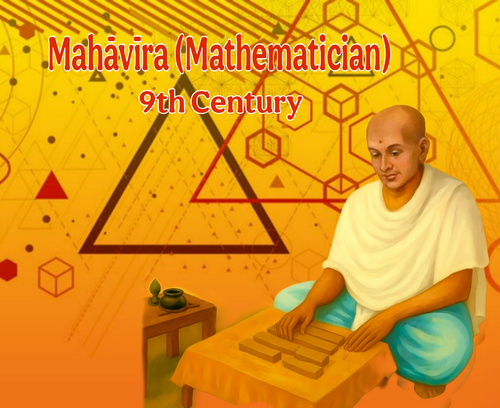
\includegraphics[width=1.0in]{images/mahavira.png}}
\caption*{\small ``There is no computation without the art of orderly enumeration.'' -- Paraphrased from Mah\={a}v\={\i}ra, \textit{Ga\d{n}itas\={a}rasa\d{n}graha} (9th century CE)}
\end{figure}

\begin{figure}[ht]       
\centerline{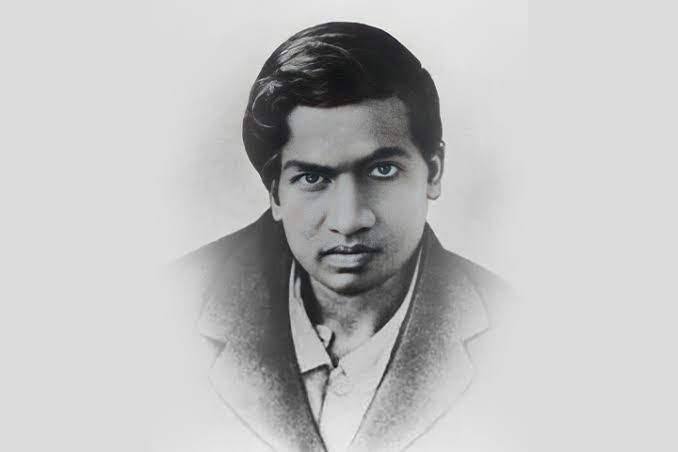
\includegraphics[width=1.0in]{images/ramanujan.jpeg}}
\caption*{\small ``There is no end to what can be counted; the more we count, the more we see patterns emerge.'' --  Paraphrased from the notebooks of Srinivasa Ramanujan}
\end{figure}


\section{Introduction}

Counting is one of the oldest and most universal human activities.
Long before the invention of symbols or written numbers, people used
stones, knots, or scratches on bones to keep track of livestock,
harvests, or trade. From these humble origins grew the entire
edifice of arithmetic, combinatorics, and probability theory.

In modern computer science and mathematics, counting is not merely an
act of enumeration but a way of understanding structure. How many
possible passwords of a given length can be formed? In how many distinct
ways can a set of vertices in a network be connected? In how many ways can certain objects be arranged? Each of these questions is,
at heart, a counting problem.

\medskip

The goal of this chapter is to develop systematic ways of counting the
number of possible outcomes in a finite discrete system, and then to
use these counts to reason about uncertainty and probability.

\begin{itemize}
  \item We first learn the \emph{basic counting principles}—the
  addition and multiplication rules—that form the backbone of all
  enumeration.
  \item We then study \emph{permutations} and \emph{combinations},
  which tell us how many ways elements can be arranged or selected.
%  \item The elegant yet deceptively powerful \emph{pigeonhole
%  principle} shows how counting can yield strong existence proofs.
\item We then study about the \emph{binomial theorem} and \emph{binomial coefficients}.
  \item Finally, we build upon these ideas to develop the foundations
  of \emph{discrete probability}—reasoning about likelihood when
  outcomes are finite and equally likely.
\end{itemize}

\section{The rules of sum and product}

\subsection{The rule of sum}
If a task can be done in $m$ ways, and another independent task can be
done in $n$ ways, and the two tasks cannot be done simultaneously,
then there are $m+n$ ways of choosing one of the two tasks.

\begin{example} 
\begin{enumerate}
\item Suppose you may take either a bus or a train to reach a city. If there
are 3 bus routes and 2 train routes, then there are $3+2=5$ ways to
travel.
\item Suppose the sections 1, 2 , and 3 of QRMT have 85, 90 and 88 students respectively. If we have to choose one class representative from the combined three sections, then there are $85 + 90 + 88 = 263$ ways
to choose the representative.
\end{enumerate}
\end{example}

\subsection{The rule of product}
If a task consists of two successive stages, the first of which can be
done in $m$ ways and the second in $n$ ways, then the entire task can
be done in $m \times n$ ways.

\begin{example}  
\begin{enumerate}
\item Suppose you must choose a shirt and a pair of trousers. If there are
4 shirts and 3 trousers, then there are $4 \times 3 = 12$ possible
outfits.
\item Suppose the sections 1, 2 , and 3 of QRMT have 85, 90 and 88 students respectively. If we have to choose one class representative from each of the three sections independently, then there are
$85 \times 90 \times 88 = 673200$ ways of choosing the three representatives.
\end{enumerate}
\end{example}

\section{Permutations}

\begin{definition}
A \emph{permutation} of a set of $n$ objects is an ordered arrangement
of all the objects. The number of permutations of $n$ objects is $n!$,
read as ``$n$ factorial'':
\[
n! = n \cdot (n-1) \cdot (n-2) \cdots 2 \cdot 1.
\]
\end{definition}

The first  can be chosen from $n$ objects, the second from the remaining $n-1$ objects, the third from the remaining $n-2$, and so on till 1.

\begin{example}
How many ways can 5 students line up for a photograph? \\
\emph{Solution:} There are $5! = 120$ possible line-ups.
\end{example}

Next, consider the number of ways of placing three balls coloured red, blue, and white in 10 boxes numbered $1,2,3,\ldots,10$, if each box can hold only one ball. The red ball can be placed in any of the 10 boxes, the blue ball can be place in any of the 9 remaining boxes, and the white ball can be placed in any of the remaining 8 boxes. Thus the total number of distinct ways to place these balls is $10 \times 9 \times 8 = 720$.

In general, if we have to place $r$ distinctly coloured balls in $n$ distinctly numbered boxes, then the number of distinct ways is
\[
n(n-1)(n-2) \cdots (n-r+1) =  \frac{n!}{(n-r)!}
\]

\begin{example}
\begin{enumerate}
\item In how many ways four examinations can be scheduled in a week so that no two examinations are scheduled on the same way? Considering the days as boxes and the examinations as distinct balls we obtain
the result as $7 \times 6 \times 5 \times 4 = 840$.
\item How many 3-digit numbers can be formed using the digits $\{1,2,3,4,5\}$ without repetition? Arguing similarly we arrive at  $5 \times 4 \times 3 = 60$.
\item How many four-digit decimal numbers can be formed without repeating the digits. This according to the above analysis is $10 \times 9 \times 8 \times 7 = 5040$. However, $9 \times 8 \times 7 = 504$ of them have 0 as the first digit. So, the number of distinct numbers that can be formed is $5040 - 504 = 4536$. We can also arrive at this result from the first principles by excluding 0 in the leading position. We then get the number of distinct numbers is $9 \times 9 \times 8 \times 7 = 4536$.
\end{enumerate}
\end{example}

An equivalent problem of placing distinct balls in boxes is that of arranging distinct objects. By permuting $r$ of $n$ distinct objects we mean to arrange $r$ of these $n$ objects in some order. For example, there are six ways to permute two out of three objects $a,b,c$. These are $ab,ba,ac,ca,bc,cb$. Arranging $r$ on $n$ objects amounts to filling $r$ positions with $r$ objects. We get the following definition:
\begin{definition}
\emph{Restricted permutations}: If only $r$ elements out of $n$ distinct elements are to be arranged, the number of permutations is
\[
P(n,r) = \frac{n!}{(n-r)!}.
\]
\end{definition}

\begin{example}
How many ways can 3 books be arranged on a shelf from a collection of 10?  
\[
P(10,3) = \frac{10!}{7!} = 720.
\]
\end{example}

\section{Counting functions and power sets}

Let us consider the problem of placing 3 distinctly coloured balls into 10 distinctly numbered boxes, but let a box hold as many balls as we wish. Since each of the red, blue, and the white ball can be placed in any of the 10 boxes the total number of ways is
\[
10 \times 10 \times 10 = 1000
\]
This is exactly the total number of functions that can be defined from the set of balls to the set of boxes.

In general, If there are $r$ distinct balls (the domain has $r$ elements) to be placed in $n$ distinct boxes (the co-domain has $n$ elements) and multiple balls can be mapped on to a box, then the total number of ways is $n^r$.

\begin{example}
Let us revisit the problem of scheduling four examinations in a week, but without any restrictions on number of examinations per day. This is exactly the problem of determining the number of functions that can be defined from the
courses to days of the week. The result is $7^4 = 2401$.
\end{example}

\begin{exercise}
Suppose that the popular tea company serve tea to their customers with 12 types of ingredients, each ingredient can be present or absent. How many different types of tea can they serve? 
\end{exercise}

\begin{exercise}
An $n$-bit binary number is defined as $b_0 + b_1 \times 2^1 + b_2 \times 2^2 + \ldots + b_{n-1} \times 2^{n-1}$, where each $b_i$ is 0 or 1. How many $n$-bit binary numbers are there? How many will have an even number of 1s?
\end{exercise}


\begin{exercise}
How many functions (truth tables) of $n$ boolean input and 1 boolean output can we define?
\end{exercise}

\subsection{Power set}
The Power set ${\cal P}(A)$ of a set $A$ is defined as the set of all subsets of $A$. For example, the set of all subsets of $A$ is ${\cal P}(A) = \left\{\phi, \left\{0\right\},  \left\{1\right\},  \left\{0,1\right\} \right\}$. Suppose the size of $A$ is
$r$. What is the size of ${\cal P}(A)$?

Consider the problem of placing each of the $r$ elements in two boxes -- inside the subset or outside. Since the $2^r$ ways of placing the $r$ elements, there are $2^r$ elements in ${\cal P}(A)$.


\section{Combinations} 

Consider now the problem of placing three balls, all red, in 10 boxes numbered $1,2,\ldots,10$. What are the total number of ways the balls can be placed if each box can hold at most one ball?

If the balls were of three shades of red, and hence distinguishable, then the answer would be $P(10,3)$. However, if  they are indistinguishable then $3!$ of the ways of their placement actually becomes one, and the number of ways reduces to $P(10,3)/3!$.

A problem equivalent to placing $r$ indistinguishable objects in $n$ numbered boxes is that of selection of $r$ objects from $n$ distinct objects. If we were to select $r$ objects from $n$, we can imagine the $n$ objects as boxes, and mark the selected ones. 

\begin{definition}
A \emph{combination} is a selection of objects without regard to order.
The number of combinations of $r$ objects chosen from $n$ is
\[
C(n,r) = \frac{n!}{r!(n-r)!}.
\]
\end{definition}
This is also sometimes denoted as $\binom{n}{r}$.

\begin{example}
\begin{enumerate}
\item Suppose Dining@Ashoka wants to schedule \emph{Tinda Kala Chana} at lunch three times a week. They can clearly do so in $\binom{7}{3} =  \frac{7!}{3!4!} = 35$ ways.
\item From 10 professors, in how many ways can a committee of 3 be chosen? The answer is $\binom{10}{3} = \frac{10!}{3! \, 7!} = 120$.
\end{enumerate}
\end{example}

\begin{exercise}
Clearly $\binom{n}{r} = \binom{n}{n-r}$. Give a combinatorial argument for the above.
 \end{exercise}
 \begin{example}
 \label{ex:rook}
Consider a $p \times q$ chess board. In how many ways a rook can move from the bottom-leftmost corner to the top-rightmost, moving only towards right and top? There are total  of $p-1$ right moves and $q-1$ top moves to be made. Think of them as red and blue balls respectively. Then, the problem is equivalent to the number of ways of choosing $p-1$ red balls from $p+q-2$ total balls, which is $\binom{p+q-2}{p-1}$. This is also exactly equal to $\binom{p+q-2}{q-1}$.
\end{example}


\begin{exercise}
Suppose we have to place $r$ balls in $n$ numbered boxes, where $q_1$ them are of one colour, $q_2$ of them are in second colour, $\ldots$, and $q_k$ of them are of the $k^{th}$ colour. Argue that the total number of ways to place the balls is
\[
\frac{P(n,r)}{q_1! q_2! \cdots q_k!}
\]
\end{exercise}

\begin{example}
\label{ex:rajan-suban}
Among 11 professors there are $C(11,5) = 462$ ways of selecting a committee of 5 members. Also, there are $C(10,4) = 210$ ways to select a committee of 5 members so that a particular professor, say professor Rajan, is always included, and there are $C(10,5) = 252$ ways of selecting a committee of 5 members so that professor Rajan is always excluded.  

We now ask in how many ways we can select a committee of 5 members so that at least one of prof Rajan and prof Suban will be included. The number of selections including both is $C(9,3) = 84$. The number of selections including Rajan but excluding Suban is $C(9,4) = 126$, as is the number of selections including Suban but excluding Rajan. Thus, the total number of ways is
\[
84+126+126 = 336
\]
Alternatively, since the total number of selections excluding both Rajan and Suban is $C(9,5)$, the total number of ways of selection is
\[
C(11,5) - C(9,5) = 462 - 126 = 336
\]
\end{example}

\subsection{Combination with repetitions}

Consider the problem of placing $r$ identical balls in $n$ numbered boxes, but allowing as many balls in a box as we wish. 

As an equivalent problem, consider the problem of arranging $n+1$ 1s and $r$ 0s with a 1 at the beginning and a 1 at the end of each arrangement. If we consider the 1s as inter-box partitions and 0s as balls, then every such arrangement is
a way of placing the $r$ balls in the $n$ boxes with possible repetitions. For example, let $ n= 5$, and $r = 4$. Then the sequence
\[
1011001101
\]
represents placing 1 ball in the first box, none in the second, 2 balls in the third box, none in the fourth, and 1 ball in the fifth box. The number of ways of arranging $r$ 0s and $n+1$ 1s with 1s at both ends is
\[
C(n+r-1,r) = \frac{(n+r-1)!}{r!(n-1)!}
\]

\begin{example}
\begin{enumerate}
\item The number of ways to select three days in a week with repetitions allowed is $C(9,3) = 84$.
\item The number of ways to select seven out of three days with repetitions allowed is $C(9,7) = 36$.
\item When three dices are rolled, the number of different outcomes is $C(8,3) = 56$.
\end{enumerate}
\end{example}
\section{The principle of Inclusion and Exclusion}

% ---------- Venn for two sets: inclusion–exclusion signs ----------
\begin{figure}[h]
\centering
\begin{tikzpicture}[scale=1.1, every node/.style={font=\small}]
  % Universe box
  \draw[rounded corners] (-3,-2) rectangle (3,2) node[anchor=south east] {$U$};

  % Circles A and B
  \def\r{1.5}
  \coordinate (cA) at (-0.9,0);
  \coordinate (cB) at ( 0.9,0);
  \draw[fill=black!8]  (cA) circle (\r);
  \draw[fill=black!8]  (cB) circle (\r);

  % Intersection hatch
  \begin{scope}
    \clip (cA) circle (\r);
    \fill[pattern=north east lines] (cB) circle (\r);
  \end{scope}

  % Set labels
  \node[anchor=south] at ($(cA)+(-0.2,\r)$) {$A$};
  \node[anchor=south] at ($(cB)+( 0.2,\r)$) {$B$};

  % PIE signs
  % Single-only regions (+)
  \node at ($ (cA)+(-0.65,0) $) {$+$};
  \node at ($ (cB)+( 0.65,0) $) {$+$};
  % Pairwise overlap (−)
  \node at ($ (cA)!0.5!(cB) $) {$-$};

  % Optional explanatory legend (comment out if not needed)
%  \node[align=left, anchor=north west] at (-2.8,-1.7) {%
%    \(\displaystyle |A\cup B|=|A|+|B|-|A\cap B|\)\\
%    \(\color{black}{+}\) singles,\ \(\color{black}{-}\) overlap
%  };
\end{tikzpicture}
\caption{The principle of inclusion and exclusion (2 sets).}
\label{fig:incl-excl-2}
\end{figure}
\begin{figure}[h]
\centering
\begin{tikzpicture}[scale=1.2, every node/.style={font=\footnotesize}]
  % Universe
  \draw[rounded corners] (-3.5,-3.0) rectangle (3.5,3.0);

  % Circle centers and radius
  \def\r{1.7}
  \coordinate (cA) at (-1,0.7);
  \coordinate (cB) at ( 1,0.7);
  \coordinate (cC) at ( 0,-1);

  % Fill each set lightly
  \draw[fill=black!10] (cA) circle (\r);
  \draw[fill=black!10] (cB) circle (\r);
  \draw[fill=black!10] (cC) circle (\r);

  % Pairwise overlaps (hatched)
  \begin{scope}
    \clip (cA) circle (\r);
    \fill[pattern=north east lines] (cB) circle (\r);
  \end{scope}
  \begin{scope}
    \clip (cA) circle (\r);
    \fill[pattern=north west lines] (cC) circle (\r);
  \end{scope}
  \begin{scope}
    \clip (cB) circle (\r);
    \fill[pattern=horizontal lines] (cC) circle (\r);
  \end{scope}

  % Triple overlap (darker)
  \begin{scope}
    \clip (cA) circle (\r);
    \clip (cB) circle (\r);
    \fill[black!30] (cC) circle (\r);
  \end{scope}

  % Set labels
  \node at ($(cA)+(0,\r+0.25)$) {$A$};
  \node at ($(cB)+(0,\r+0.25)$) {$B$};
  \node at ($(cC)+(0,-\r-0.20)$) {$C$};

  % Inclusion-Exclusion sign pattern
  \node at ($(cA)+(-0.9,0.1)$) {$+$};
  \node at ($(cB)+( 0.9,0.1)$) {$+$};
  \node at ($(cC)+( 0.0,-1.0)$) {$+$};

  \node at ($ (cA)!0.5!(cB) + (0,0.3) $) {$-$};
  \node at ($ (cA)!0.5!(cC) + (-0.3,-0.1) $) {$-$};
  \node at ($ (cB)!0.5!(cC) + (0.3,-0.1) $) {$-$};

  \node at ($(cA)!0.35!(cC)!0.5!(cB)$) {$+$};

  % Caption formula
%  \node[anchor=north west, align=left] at (-3.1,-2.3) {%
%    $|A\cup B\cup C| =$\\
%    $\quad |A|+|B|+|C|$\\
%    $\quad -(|A\cap B|+|A\cap C|+|B\cap C|)$\\
%    $\quad +|A\cap B\cap C|$};

\end{tikzpicture}
\caption{The principle of inclusion and exclusion (3 sets).}
\label{fig:incl-excl-3}
\end{figure}

The problem of Example \ref{ex:rajan-suban} can also be solved by the following method. Among the 462 ways of selecting the committee of 5, let $A_1$ and $A_2$ be the set of ways of selection that include Rajan and Suban respectively.  Now, since
\[
\begin{array}{l}
\mid A_1 \mid = C(10,4) = 210 \\
\mid A_2 \mid = C(10,4) = 210 \\
\mid A_1 \cap A_2 \mid = C(9,3) = 84 \\
\end{array}
\]
We. can estimate $\mid A_1 \cup A_2 \mid$, the number ways to include at least one of Rajan and Suban, as 
\[
\mid A_1 \cup A_2 \mid = \mid A_1 \mid + \mid A_2 \mid - \mid A_1 \cap A_2 \mid  = 210+210-84 = 336
\]
The last subtraction is necessary because the number of ways where both Rajan and Suban are included is double counted in $\mid A_1 \mid + \mid A_2 \mid$.  This method of counting is called the \emph{principle of inclusion and exclusion}.

For any two finite sets $A$ and $B$,
\[
|A \cup B| = |A| + |B| - |A \cap B|.
\]
The subtraction corrects for the double counting of elements common to both sets (See Figure \ref{fig:incl-excl-2}) .

\begin{example}
Let $A$ be the set of students taking Mathematics (40 students) and
$B$ be those taking Physics (30 students), with 10 students taking
both. Then, the size of the set taking at least one of Mathematics and Physics is
\[
|A \cup B| = 40 + 30 - 10 = 60.
\]
\end{example}


For three finite sets $A,B,C$,
\[
|A \cup B \cup C| =
|A| + |B| + |C|
- |A \cap B| - |A \cap C| - |B \cap C|
+ |A \cap B \cap C|.
\]

\begin{exercise}
Argue the correctness of the above formula (see Figure \ref{fig:incl-excl-3}).
\end{exercise}

We can generalize the above for $n$ sets $A_1, A_2, \ldots, A_n$ as,
\[
\left|\bigcup_{i=1}^{n} A_i\right|
= \sum_{i} |A_i|
- \sum_{i<j} |A_i \cap A_j|
+ \sum_{i<j<k} |A_i \cap A_j \cap A_k|
- \cdots + (-1)^{n+1} |A_1 \cap A_2 \cap \cdots \cap A_n|.
\]

\begin{example}[Derangements]
How many permutations of $\{1,2,3\}$ have no fixed point (i.e., no
element appears in its original position)?  
Let $A_i$ denote the set of permutations that fix $i$.  
\[
|A_1|=|A_2|=|A_3|=2,\quad
|A_i \cap A_j|=1,\quad
|A_1 \cap A_2 \cap A_3|=1.
\]
Thus,
\[
|\overline{A_1 \cup A_2 \cup A_3}| =
3! - (3\times2) + (3\times1) - 1 = 6 - 6 + 3 - 1 = 2.
\]
Hence, there are 2 derangements.
\end{example}

\begin{example}
Suppose an Ashoka student wants to make up a schedule for a seven-day period during which she will study only one subject each day. She is taking four subjects - Environmental Studies (EVS), Great Books (GB), Economic Politics and Society (EPS) and Quantitative Reasoning and Mathematical Thinking (QRMT). Clearly, there are $4^7$ different schedules. We want to know the number of schedules that devote at least one day to each subject?

Let $A_1$ denote the set of schedules in which EVS is never studied; likewise $A_2$, $A_3$, $A_4$ for GB, EPS, and QRMT respectively. Then,
\[
A_1 \cup A_2  \cup A_3  \cup A_4
\]
is the set of schedules in one or more of the subjects is not included.
Since
\[
\begin{array}{l}
\mid A_1 \mid = \mid A_2  \mid = \mid A_3  \mid =  \mid A_4 \mid = 3^7 \\
\mid A_1 \cap A_2 \mid = \mid A_1 \cap A_3 \mid = \mid A_1 \cap A_4 \mid = \mid A_2 \cap A_3 \mid =  \mid A_2 \cap A_4 \mid = \mid A_3 \cap A_4 \mid = 2^7 \\
\mid A_1 \cap A_2 \cap A_3 \mid = \mid A_1 \cap A_2 \cap A_4 \mid =  \mid A_1 \cap A_3 \cap A_4 \mid = \mid A_3 \cap A_3 \cap A_4 \mid = 1^7 \\
\mid A_1 \cap A_2 \cap A_3 \cap A_4 \mid = 0 \\
\end{array}
\]
We obtain
\[
\mid A_1 \cup A_2  \cup A_3  \cup A_4 \mid = 4(3^7) - 6(2^7) + 4
\]
\end{example}
Consequently, the number of schedules in which all subjects will be included is
\[
4^7 - (4(3^7) - 6(2^7) + 4)
\]
\begin{exercise}
Convince yourself $P(7,4)*4^3$ -- there are $P(7,4)$ ways to schedule 4 subjects for 4 of the 7 days, and $4^3$ ways to schedule three subjects for the remaining three days -- is not the correct answer.
\end{exercise}

\section{Recurrences: Counting by Relations}

Consider the following algorithms for sorting a list of integers in ascending order. Suppose we start with a sequence in random order such as
\[
\mid 8 \;3\;5\;9\;7
\] 
The symbol $\mid$ denotes that the elements to the right are unsorted. At the first step we can search through the list for the minimum element, and swap it with the element in the first position. We obtain a sorted part and an unsorted part
\[
3\mid8\;5\;9\;7
\]
Then, keeping the sorted part fixed, we can search through the rest of the list for the minimum element and swap it with the first element in the unsorted part to obtain
\[
3\;5\mid8\;9\;7
\]
Repeating the process we obtain in a sequence
\[
3\;5\;7\mid 9\;8
\]
and
\[
\begin{array}{l}
3\;5\;7\;8\mid 9 \\
3\;5\;7\;8\; 9 \mid
\end{array}
\]
Our problem is to count the number of comparisons required to sort a random sequence of $n$ elements.  

We can do this using the principle of mathematical induction. Let $T(n)$ be the number of comparisons required to solve a sorting problem of size $n$. If $n = 1$ then the sequence is sorted by default. Otherwise, we need to search
through $n$ elements to find the minimum which requires $n - 1$ comparisons, and are left with an identical subproblem of size $n-1$ which forms the induction hypothesis $T(n-1)$. Hence,
\[
T(n) = \left\{ 
            \begin{array}{ll}
            0 & \mbox{if $n = 1$} \\
            T(n-1) + (n-1) & \mbox{if $n > 1$}
            \end{array}
           \right.
\]
The above is called a \emph{recurrence relation}. We can solve this by telescoping
\[
\begin{array}{lll}
T(n) & = & T(n-1) + (n-1) \\
        & = & T(n-2) + (n-2) + (n-1) \\
        & \vdots & \vdots \\
         & = & T(1) + 1 + 2 + \ldots + (n-1) \\
         & = &  1 + 2 + \ldots + (n-1) = n(n-1)/2
\end{array}
\]
Thus we require $n(n-1)/2$ comparisons.


A \emph{recurrence relation} defines a sequence by relating each term to earlier ones.
Recurrences arise naturally in counting when a choice splits a problem into
smaller subproblems.  In fact, all counting problems can be expressed through recurrences. Consider the following examples.

\begin{example}
Consider the counting problem of number of distinct ways of arranging $n$ objects. There is only one way to arrange an empty set of objects, which forms the base case $P(0) = 1$. Suppose $P(n-1)$ is the number of ways
of arranging $n-1$ objects for $n > 0$ (the induction hypothesis). Then, the $n^{th}$ object can be inserted in each of the $P(n-1)$ arrangements in $n$ ways. Thus we have
\[
P(n) = \left\{ 
            \begin{array}{ll}
            1 & \mbox{if $n = 0$} \\
            n * P(n-1)  & \mbox{if $n > 0$}
            \end{array}
           \right.
\]

which evaluates to $P(n) = n!$
\end{example}
\begin{example}
Consider the rook problem of Example \ref{ex:rook}. In how many ways a rook can move from the bottom-leftmost corner to the top-rightmost in a $p \times q$ chessboard, moving only towards right and top? If $p = 1$ or $q = 1$ (a 1-dimensional chessboard), then there clearly is only one way giving us our base case. Otherwise, by the rule of sum, it is the sum of the total number of ways by taking the first step towards the right and the total number of ways by taking the first step towards the top. We obtain
\[
Rook(p,q) = \left\{ 
            \begin{array}{ll}
            1 & \mbox{if $p = 1$ or $q = 1$} \\
             Rook(p-1,q) + Rook(p,q-1) & \mbox{otherwise}
            \end{array}
           \right.
\]
Note that $Rook(p-1,q)$ and $Rook(p,q-1)$ are identical subproblems of smaller sizes, and hence are valid induction hypotheses. We saw earlier that this must be equal to $\binom{p+q-2}{p-1} = \binom{p+q-2}{q-1}$.
\end{example}

\subsection{\href{https://mathworld.wolfram.com/PascalsTriangle.html}{Pascal's triangle}}
The fact that the above recurrence evaluates to a combination suggests that  combination may itself be expressed as a recurrence. Consider the problem of selecting $r$ identical balls from $n$ boxes without repetition. Clearly,
if $r=0$ or $r=n$ we have exactly one way, giving our bases cases as $C(n,0) = C(n,n) = 1$. Now, by the rule of sum, the total number of ways of selecting is equal to the sum of the total number of ways of selecting by picking one from the $n^{th}$ box and the total number of ways by not picking at all from the $n^{th}$ box. This gives us
\[
C(n,r) = \left\{ 
            \begin{array}{ll}
            1 & \mbox{if $r = 0$ or $r = n$} \\
             C(n-1,r-1) + C(n-1,r) & \mbox{otherwise}
            \end{array}
           \right.
\]

The above recurrence leads us to the famous triangle of numbers called the \href{https://mathworld.wolfram.com/PascalsTriangle.html}{Pascal's triangle}\footnote{The triangular arrangement of binomial coefficients is commonly associated
with Blaise Pascal, whose posthumous work (1665) presented it systematically.
However, the structure was known much earlier. The Italian algebraist 
Niccol\`o Tartaglia published its first six rows in 1556. Even earlier, it
appeared in the writings of the Chinese mathematician Y\`ang Hu\`i and in the
work of the Persian scholar Omar Khayy\=am. Consequently, the triangle is known
by different names in different traditions:  Y\`ang Hu\`i triangle in China,
Khayy\=am's triangle in Persia, and Tartaglia's triangle in Italy.}.

Starting with $n=0$ the triangle is
\[
\begin{array}{lllllll}
1 \\
1 & 1 \\
1 & 2 & 1 \\
1 & 3 & 3  & 1 \\
1 & 4 & 6  & 4  & 1 \\
1 & 5 & 10 & 10 & 5 & 1 \\
1 & 6 & 15  & 20  & 15 &  6 &  1 
\end{array}
\]
Note that each number $\binom{n}{r}$ can be obtained by adding the two to the top and left in the previous row. Instead of computing $n!$ and $r!$ which are rather inefficient, the triangle gives faster method of computing $\binom{n}{r}$.

\begin{exercise}
A curious fact about the Pascal's triangle is that is we start from each of the 1s in the first column and add up the numbers along the anti-diagonals (in the direction $\nearrow$), then we obtain the Fibonacci numbers.  For example
\[
\begin{array}{l}
1 \\
1 \\
1 + 1 = 2\\
1 + 2 = 3 \\
1 + 3 + 1 = 5 \\
1 + 4 + 3 = 8 \\
1 + 5 + 6 + 1 = 13 \\
1 + 6 + 10 + 4 = 21 \\
\vdots
\end{array}
\]

Can you figure out why?
\end{exercise}

\begin{example}
 A shop keeper in the Asawarpur village adjoining Ashoka university thought of the following problem: 
      how many ways can one make a change of \rupee 1, given coins of 
      denomination 50p, 25p, 10p, 5p and 1p? More generally, can one write a 
      function to compute the number of ways to change any given amount of 
      money?  After giving some thought to the problem she noted that the 
      total number of ways to make change for some amount is equal to the 
      number of ways to make change for the amount without using any of the 
      first kind of coin, plus the number of ways to make change assuming we 
      do use a coin of the first kind. But the latter number is equal to the 
      number of ways to make change for the amount that remains after using 
      one coin of the first kind.  With this solution in mind she approached 
      the students of QRMT  for a recurrence for the problem. 
      Assume that there is a 
      function $d: \N \rightarrow \N$ that given you the denomination
      of the $n^{th}$ type of coin (for example, $d(1) = 1$, $d(2)=25$, $d(3) = 10$, $d(4)=5$ and
      $d(5) = 50$)\footnote{This is a special case of a general class of problems called the \href{https://en.wikipedia.org/wiki/Integer_partition}{partition problem}}.
\end{example}
\begin{exercise}
Suppose the amount for which change has to be generate is $a$. Argue that a solution to the counting problem is given by the following recurrence.
\[
Coin(a,n) = \left\{ 
            \begin{array}{ll}
            0 & \mbox{if $a < 0$ or $n = 0$} \\
             Coin(a,n-1) + Coin(a-d(n),n) & \mbox{otherwise}
            \end{array}
           \right.
\]

\end{exercise}


\section{The Binomial Theorem}\label{sec:binomial-theorem}

When we expand an expression of the form $(x+y)^n$ for a positive integer $n$,
we obtain a sum of products involving powers of $x$ and $y$. For small $n$, we
can compute these expansions by hand:
\[
(x+y)^2 = x^2 + 2xy + y^2, \qquad
(x+y)^3 = x^3 + 3x^2y + 3xy^2 + y^3.
\]
A clear pattern emerges: each term consists of a power of $x$ multiplied by a
power of $y$, and the coefficients follow the rows of Pascal's triangle. The
binomial theorem makes this pattern precise, expressing $(x+y)^n$ as a sum in
which the coefficients are exactly the binomial numbers $\binom{n}{k}$.

\begin{theorem}[Binomial Theorem]
For any integer $n \ge 0$ and for all commuting symbols or numbers $x,y$,
\[
(x+y)^n = \sum_{k=0}^{n} \binom{n}{k}\, x^{\,n-k} y^{\,k}.
\]
\end{theorem}

\begin{proof} ({\bf A combinatorial proof})
Expand $(x+y)^n$ as a product of $n$ identical factors:
\[
(x+y)^n = (x+y)(x+y)\cdots(x+y).
\]
A term $x^{\,n-k}y^{\,k}$ is formed by choosing $y$ from exactly $k$ of the $n$
factors and choosing $x$ from the remaining $n-k$ factors. The number of ways to
choose which $k$ factors contribute the $y$ is $\binom{n}{k}$. Thus,
\[
(x+y)^n = \sum_{k=0}^{n} \binom{n}{k}\, x^{\,n-k} y^{\,k}.
\]
\end{proof}

\begin{proof} ({\bf An inductive proof})
We prove the identity by induction on $n$.

\emph{Base case:} $n=0$. $(x+y)^0 = 1$ agrees with the right-hand side.

\emph{Inductive step:} 
Assume that for some $n \ge 0$,
\[
(x+y)^n = \sum_{k=0}^{n} \binom{n}{k} x^{\,n-k} y^{\,k}. \tag{$\ast$}
\]
We prove the identity for $n+1$.

\[
(x+y)^{n+1}
= (x+y)(x+y)^n
= (x+y)\sum_{k=0}^{n} \binom{n}{k} x^{\,n-k} y^{\,k}.
\]

Distribute:
\[
(x+y)^{n+1}
= \sum_{k=0}^{n} \binom{n}{k} x^{\,n+1-k} y^{\,k}
  + \sum_{k=0}^{n} \binom{n}{k} x^{\,n-k} y^{\,k+1}. \tag{1}
\]

We now \emph{reindex} the second sum. Let $j = k+1$. Then when $k=0$, $j=1$,
and when $k=n$, $j=n+1$. Also $k = j-1$. Therefore:
\[
\sum_{k=0}^{n} \binom{n}{k} x^{\,n-k} y^{\,k+1}
= \sum_{j=1}^{n+1} \binom{n}{\,j-1\,} x^{\,n-(j-1)} y^{\,j}
= \sum_{j=1}^{n+1} \binom{n}{\,j-1\,} x^{\,n+1-j} y^{\,j}. \tag{2}
\]

Now substitute $(2)$ into $(1)$ and combine the sums by matching powers:
\[
(x+y)^{n+1}
= \binom{n}{0} x^{\,n+1}
  + \sum_{j=1}^{n} \left(\binom{n}{j} + \binom{n}{j-1}\right) x^{\,n+1-j} y^{\,j}
  + \binom{n}{n} y^{\,n+1}. \tag{3}
\]

\medskip
Finally, we apply \textbf{Pascal's identity}:
\[
\binom{n}{j} + \binom{n}{j-1} = \binom{n+1}{j}.
\]

Substituting this into $(3)$ gives:
\[
(x+y)^{n+1}
= \sum_{j=0}^{n+1} \binom{n+1}{j} x^{\,n+1-j} y^{\,j}.
\]

This is exactly the binomial expansion for $(x+y)^{n+1}$, completing the induction.
\[
\boxed{(x+y)^n = \sum_{k=0}^{n} \binom{n}{k} x^{\,n-k} y^{\,k} \text{ for all } n \ge 0.}
\]
\end{proof}

\subsection*{Corollaries}
\begin{enumerate}
  \item $(1+1)^n = \sum_{k=0}^{n}\binom{n}{k} = 2^{n}$. (Give a purely combinatorial argument for this identity.)
  \item $(1-1)^n = \sum_{k=0}^{n}(-1)^k\binom{n}{k} = 0$ for $n \ge 1$.
  \item The coefficient of $x^{\,n-k}y^{\,k}$ in $(x+y)^n$ is $\binom{n}{k}$.
\end{enumerate}

\begin{example}
Using the binomial theorem,
\[
(2x - 3)^4
= \sum_{k=0}^{4} \binom{4}{k} (2x)^{4-k} (-3)^k
= 16x^4 - 96x^3 + 216x^2 - 216x + 81.
\]
\end{example}

\section{Discrete Probability}

Probability provides a mathematical language for reasoning about uncertainty.
Everyday situations such as tossing a coin, rolling a die, shuffling cards,
choosing passwords, or hashing data involve outcomes that cannot be predicted
with certainty in advance. Yet, they are not completely unpredictable: the set
of all possible outcomes is known, and many useful questions concern the
\emph{likelihood} of particular events. In this section we develop a framework
for thinking systematically about such situations.

We begin by describing random experiments and their sample spaces, and how
events are formed from outcomes. We then introduce probability measures and the
basic axioms that govern them. Next, we discuss random variables, which allow
us to assign numerical values to outcomes and reason about distributions,
independence, and conditional probabilities. Bayes' theorem provides a powerful
tool for updating beliefs in the light of new information. Finally, we conclude
with the concepts of information and entropy, which quantify uncertainty and
play a central role in modern data science, coding theory, and learning systems.

\subsection{Experiments, Sample Spaces, and Events}

A \emph{random experiment} is a process whose outcome cannot be predicted with
certainty in advance, even though all possible outcomes are known.
The set of all possible outcomes is called the \emph{sample space}, denoted $S$.
An \emph{event} is a subset $E \subseteq S$.

\begin{example}
\begin{enumerate}
  \item Tossing a fair coin: $S = \{\text{H}, \text{T}\}$.
  \item Rolling a fair die: $S = \{1,2,3,4,5,6\}$.
  \item Drawing a card from a standard deck of 52 cards.
\end{enumerate}
\end{example}

Two events $A$ and $B$ are \emph{mutually exclusive} if $A \cap B=\varnothing$.
A collection of events $A_1, \dots, A_k$ is \emph{exhaustive} if
$A_1 \cup A_2 \cup \cdots \cup A_k = S$.

\subsection{Probability Measure and Axioms}

A \emph{probability measure} assigns to each event $E\subseteq S$ a number
$P(E)$ satisfying:
\[
P(E)\ge 0,\qquad P(S)=1,\qquad.
\]

When $S$ is finite and all outcomes are equally likely,
\[
P(E)=\frac{|E|}{|S|}.
\]

\begin{example}
\begin{enumerate}
  \item $P(\text{even number when rolling a die}) = \frac{3}{6} = \frac{1}{2}$.
  \item $P(\text{ace from a deck}) = \frac{4}{52} = \frac{1}{13}$.
  \item Consider the problem of dealing a poker hand out of a deck of cards. The sample space consists of $C(52,5)$ different hands that can be dealt. We assume that all of these are equally probable. What is the
          probability of getting four aces? We note that 48 possible outcomes from the sample space contain 4 aces (1 way to choose 4 aces and 48 ways to choose the remaining card). So, the probability is
          $48/C(52,5) = 0.0000185$.
  \item What is the probability that in the QRMT class of 88 students, no two have the same birthday (assuming no leap year)? Each of the 88 students can have their birthdays in 365 ways, so the sample space is $365^{88}$.Out of
           these $P(365,88)$ correspond to the distribution of birthdays so that no two are the same. So, the probability that no two have the same birthday is $P(365,88)/365^{88} \approx 10^{-5}$, which is rather small. Hence, the probability is close to 1 (almost certain) that at least two people have the same birthday. For how many students is the probability nearly 0.5?
  \item Suppose 8 Ashoka students are in a tug-of-war team. What is the probability that there are exactly two from each of the four years? Clearly, the sample space is of size $4^8$. The total number of ways to select exactly two from each batch is $8!/(2!2!2!2!)$. So the probability is
  \[
    \frac{8!}{2!2!2!2!4^8} = 0.0385
  \]
\item Consider the experiment of shooting a target until there is a hit where the probability of a hit or a miss in a single shot is 1/2 (not a very good shooter). The, the probability of $k$ misses before a hit is $2^{-(k+1)}$. Let
$A$ denote the event that there is a hit in no more than 5 misses. Then $A = \{h,mh,mmh,mmmh,mmmmh,mmmmmh\}$. Thus
\[
P(A) = \sum_{k=0}^5 2^{-(k+1)} = 0.984
\]
Let $B$ denote the event that there is a hit after odd number of misses. Then\footnote{We will study the methods to evaluate such infinite summations in Section \ref{sec:apgp}.},
\[
P(B) = \sum_{i=1}^\infty 2^{-2i} = 1/3
\]
On the other  hand, if $C$ is the event that there is a hit after an even number of misses, then
\[
P(C) = \sum_{i=1}^\infty 2^{-2i+1} = 2/3
\]
\end{enumerate}
\end{example}

\subsection{Random Variables, probability distribution, expectation and variance}

A \emph{random variable} is a function
\[
X : S \longrightarrow \mathbb{R}.
\]
It assigns a numerical value to each outcome of the experiment.

\begin{example}
If $S=\{1,2,3,4,5,6\}$, then $X(\omega)=\omega$ simply records the number rolled.
\end{example}

The \emph{distribution} of $X$ is given by
\[
P(X=x)=|\{\omega\in S : X(\omega)=x\}|/|S|.
\]


The \emph{expectation} or \emph{expected value} of a discrete random variable
$X$ is the weighted average of its possible values, where each value is
weighted by its probability. It captures the \emph{long-run average} or the \emph{mean} outcome
if the experiment is repeated many times.

Let $X$ take values $x_1, x_2, \dots, x_n$ with probabilities
$P(X=x_i)$, or more generally let $X$ take countably many values.
Then the expectation of $X$ is defined as
\[
\mathbb{E}[X] = \sum_{x} x \, P(X=x).
\]

\paragraph{Interpretation.}
If we repeat the experiment many times and record the values of $X$, the
average of the recorded values will be close to $\mathbb{E}[X]$.
Thus, expectation represents the \emph{typical} or \emph{average}
outcome in the long run.

\begin{example}
\begin{enumerate}
  \item \textbf{Fair Die.}  
  The random variable $X$ equals the number rolled:
  \[
  \mathbb{E}[X]
  = \frac{1}{6}(1+2+3+4+5+6)
  = \frac{21}{6}
  = 3.5.
  \]
  The expected value need not be a possible outcome.

  \item \textbf{Indicator Variables.}  
  If $I_A$ is the indicator of event $A$ (i.e., $I_A=1$ if $A$ occurs and
  $0$ otherwise), then
  \[
  \mathbb{E}[I_A] = P(A).
  \]
  So expectations generalize probabilities.
\end{enumerate}
\end{example}

\begin{example}
Consider rolling two fair six-sided dice. Let $X$ be the value on the first die
and $Y$ the value on the second die. Define the random variable
\[
S = X + Y,
\]
the \emph{sum} of the two dice.

Since each die has 6 faces and the dice are independent, the sample space
consists of $36$ equally likely ordered pairs:
\[
S = \{(1,1), (1,2), \dots, (6,6)\}, \qquad P((i,j)) = \frac{1}{36}.
\]

The possible values of the sum $S$ range from $2$ to $12$.
To compute $P(S = s)$, we count how many ordered pairs $(i,j)$ satisfy $i+j=s$.

\[
P(S = s)=\frac{\mid\{(i,j):\, i+j=s\}\mid}{36}.
\]

The number of such pairs increases from $s=2$ up to $s=7$, then decreases symmetrically:

\[
P(S = s)=
\begin{cases}
\frac{s-1}{36}, & 2 \le s \le 7,\\[6pt]
\frac{13-s}{36}, & 8 \le s \le 12.
\end{cases}
\]

\paragraph{Distribution Table.}  
\[
\begin{array}{c|ccccccccccc}
s & 2 & 3 & 4 & 5 & 6 & 7 & 8 & 9 & 10 & 11 & 12 \\ \hline
\text{number of pairs }(i,j) & 1 & 2 & 3 & 4 & 5 & 6 & 5 & 4 & 3 & 2 & 1 \\
P(S=s) & \frac{1}{36} & \frac{2}{36} & \frac{3}{36} & \frac{4}{36} &
\frac{5}{36} & \frac{6}{36} & \frac{5}{36} & \frac{4}{36} &
\frac{3}{36} & \frac{2}{36} & \frac{1}{36}
\end{array}
\]

\paragraph{Explanation.}
The value $S=7$ is the most likely because there are more pairs of dice that add
to $7$ than to any other sum:
\[
(1,6), (2,5), (3,4), (4,3), (5,2), (6,1).
\]
There are $6$ such pairs, giving $P(S=7)=6/36=1/6$.

The distribution is symmetric because $(i,j)$ and $(j,i)$ contribute to sums
equally. Values near the center have the largest number of combinations, while
values near the extremes have fewer.
\end{example}
\begin{example}
Suppose we repeat an experiment consisting of independent identical trials,
each of which results in a \emph{success} with probability $p$ and a
\emph{failure} with probability $1-p$, where $0<p\le 1$.

Let $T$ be the random variable defined as:
\[
T = \text{the number of trials until the first success occurs}.
\]

Thus $T$ takes values in $\{1,2,3,\dots\}$.

\paragraph{Probability Distribution.}
For the first success to occur on trial $k$, the first $k-1$ trials must be
failures (each with probability $1-p$), and the $k$-th trial must be a success.

\[
P(T = k) = (1-p)^{k-1} \, p, \qquad k=1,2,3,\dots
\]

This distribution is called the \emph{Geometric distribution} with parameter $p$.

\paragraph{Verification.}
The probabilities sum to $1$\footnote{We will study the methods to evaluate such infinite summations in Section \ref{sec:apgp}.}:
\[
\sum_{k=1}^{\infty} (1-p)^{k-1} p 
= p \sum_{k=0}^{\infty} (1-p)^k
= p \cdot \frac{1}{1-(1-p)}
= 1.
\]

\paragraph{Expected Value.}
\[
\mathbb{E}[T]
= \sum_{k=1}^{\infty} k \, (1-p)^{k-1} p
= \frac{1}{p}.
\]

Thus, the average number of trials needed to get a success is $\dfrac{1}{p}$.

\paragraph{Example.}
If the probability of success on each trial is $p=\tfrac{1}{4}$ (for example,
getting a four when rolling a die), then
\[
\mathbb{E}[T] = \frac{1}{p} = 4.
\]
On average, one must roll the die $4$ times to get the first four.
\end{example}

While the expectation of a random variable measures its average value,
the \emph{variance} measures how much the values of the random variable
tend to spread out around the mean.

Let $X$ be a discrete random variable with expectation $\mu = \mathbb{E}[X]$.
The \emph{variance} of $X$ is defined as
\[
\mathrm{Var}(X)
    = \mathbb{E}\big[(X - \mu)^2\big].
\]
The quantity $(X-\mu)^2$ measures the squared deviation of $X$ from its
mean, and the expectation averages this deviation over all outcomes.

\medskip
The square root of the variance is called the \emph{standard deviation}:
\[
\sigma = \sqrt{\mathrm{Var}(X)}.
\]

Often it is easier to compute variance using the identity
\[
\mathrm{Var}(X)
= E[X^2] - (E[X])^2.
\]
This follows by expanding $(X-\mu)^2 = X^2 - 2\mu X + \mu^2$ and taking
expectation.
\subsection{The Bernoulli Distribution}

\subsubsection{Introduction}
Many experiments in probability have only two possible outcomes — such as
\emph{success/failure}, \emph{yes/no}, or \emph{head/tail}. The simplest
random variable that models such an experiment is called a
\emph{Bernoulli random variable}.

\subsubsection{Definition}
A random variable $X$ is said to have a \emph{Bernoulli distribution}
with parameter $p$ (where $0 \le p \le 1$) if
\[
P(X=1)=p \quad \text{and} \quad P(X=0)=1-p.
\]
We write this as
\[
X \sim \text{Bernoulli}(p).
\]
Here $X=1$ represents ``success'' and $X=0$ represents ``failure''.

\subsubsection{Probability Mass Function}
The probability mass function (PMF) of $X$ can be compactly expressed as
\[
P(X=x)=p^x(1-p)^{1-x}, \qquad x \in \{0,1\}.
\]

\subsubsection{Expectation and Variance}
The \emph{expected value} (mean) and \emph{variance} of a Bernoulli random
variable are
\[
E[X] = p, \qquad \text{Var}(X) = p(1-p).
\]
\emph{Proof:}
\[
E[X] = (0)(1-p) + (1)(p) = p,
\]
and
\[
E[X^2] = (0^2)(1-p) + (1^2)(p) = p.
\]
Therefore
\[
\text{Var}(X) = E[X^2] - (E[X])^2 = p - p^2 = p(1-p).
\]

\subsubsection{Example}
Consider a fair coin toss where success is ``getting a head''.
Then $p=\tfrac{1}{2}$ and
\[
P(X=1)=P(X=0)=\tfrac{1}{2}.
\]
Hence $E[X]=\tfrac{1}{2}$ and $\text{Var}(X)=\tfrac{1}{4}$.

\subsubsection{Remarks}
\begin{itemize}
  \item The Bernoulli distribution is the simplest discrete distribution.
  \item The sum of $n$ independent Bernoulli($p$) random variables follows
        a \emph{Binomial} distribution $\text{Binomial}(n,p)$.
  \item Many random processes—such as coin tossing, system reliability,
        and binary classification—are modeled as Bernoulli trials.
\end{itemize}


\subsection{Independence}

Two events $A$ and $B$ are independent if
\[
P(A\cap B)=P(A)P(B)
\]

Two random variables $X$ and $Y$ are independent if for all $x,y$,
\[
P(X=x, Y=y)=P(X=x)\,P(Y=y).
\]

\begin{example}
\begin{enumerate}
\item Consider two independent coin tosses. The sample space is  $S = \{hh,ht,th,tt\}$. If $P(h) = P(t) = 1/2$ for each toss, then $P(hh) = P(ht) = P(th) = P(tt) = 1/4$.
\item Let $X =$ result of die 1, $Y =$ result of die 2.
Then $X$ and $Y$ are independent:
\[
P(X=4, Y=2)=\frac{1}{6}\cdot\frac{1}{6}.
\]
\item  Roll two fair dice. Let
\[
A = \{\text{the first die shows a } 4\}, \qquad
B = \{\text{the second die shows an even number}\}.
\]
Then
\[
P(A)=\frac{1}{6},\qquad P(B)=\frac{1}{2}.
\]
Since the dice are independent,
\[
P(A \cap B)=P(\text{first die is }4 \text{ and second die is even})
= \frac{1}{6}\cdot \frac{1}{2} = \frac{1}{12}.
\]

\item Select one card uniformly from a standard 52-card deck. Let
\[
C = \{\text{the card is red}\}, \qquad
D = \{\text{the card is a Heart}\}.
\]
Then:
\[
P(C)=\frac{26}{52}=\frac{1}{2},\qquad
P(D)=\frac{13}{52}=\frac{1}{4}.
\]
However,
\[
P(C \cap D)=P(\text{the card is a red Heart}) = \frac{13}{52}=\frac{1}{4}.
\]
But
\[
P(C)\,P(D)=\frac{1}{2}\cdot\frac{1}{4}=\frac{1}{8}.
\]

The events $C$ and $D$ are \emph{not} independent.  Knowing that the card is a Heart \emph{already implies} that it is red.
So the occurrence of $D$ changes the probability of $C$.
\end{enumerate}
\end{example}



\subsection{Conditional Probability}

In many situations, additional information is available about the outcome of
an experiment. Such information can change the likelihood of events. The idea
of \emph{conditional probability} allows us to update probabilities when we
learn that some event has already occurred.

If $P(B)>0$, $P(A\mid B)$ is the probability of $A$ given that $B$ has occurred is given as
\[
P(A\mid B)=\frac{P(A\cap B)}{P(B)}.
\]


\begin{example}
Let $A=$ “card is a King”, $B=$ “card is a face card”.
Then
\[
P(A\mid B) = \frac{4/52}{12/52} = \frac{1}{3}.
\]
\end{example}

\subsubsection{Bayes' Theorem}

\[
P(A \mid B)=\frac{P(B\mid A)P(A)}{P(B)}.
\]
More generally, if $\{A_1,\dots,A_k\}$ partitions $S$,
\[
P(A_i\mid B)=\frac{P(B\mid A_i)P(A_i)}{\sum_{j=1}^{k}P(B\mid A_j)P(A_j)}.
\]

\begin{example}
\begin{enumerate}
\item A disease has a probability  $P(D)=0.01$.
A test has a probability $P(\text{positive}\mid D)=0.99$ and $P(\text{positive}\mid \overline{D})=0.05$.
\[
P(D\mid\text{positive})
=\frac{0.99\cdot 0.01}{0.99\cdot0.01+0.05\cdot0.99}
\approx 0.166.
\]
\item A coin was chosen at random and tossed. The probability that a fair coin was chosen  and head shows is 1/3.  The probability that a fair coin was chosen  and tail shows is  also 1/3. The probability that an unfair coin was chosen  and head shows is 1/12. The probability that an unfair coin was chosen  and head shows is 1/4. 

Clearly, the probability that head shows is
\[
\frac{1}{3} + \frac{1}{12} =  \frac{5}{12}
\]
and the probability that an unfair coin was chosen is 
\[
\frac{1}{12} + \frac{1}{4} =  \frac{1}{3}
\]
Thus, the conditional probability that an unfair coin was chosen given that head shows is
\[
\frac{1/12}{5/12}  =  \frac{1}{5}
\]
and the conditional probability that head shows given an unfair coin was chosen is
\[
\frac{1/12}{1/3}  =  \frac{1}{4}
\]
\item Three dice were rolled. Given that no two faces were the same, what is the probability that there was an ace? Let $A$ denote the event that there was an ace, and $B$ the event that no two faces were the same. Note that
\[
P(B) = \frac{P(6,3)}{6^3} \;\;\;\;\; P(A \cap B) =  \frac{3P(5,2)}{6^3}
\]
Hence,
\[
P(A \mid B) =  \frac{3P(5,2)}{P(6,3)} = \frac{1}{2}
\]
\end{enumerate}
\end{example}
%\subsection{Information and Entropy}
%
%The \emph{information content} of an event with probability $p$ is
%\[
%I(p) = -\log_2 p.
%\]
%
%A random variable $X$ with distribution $p(x)$ has \emph{entropy}
%\[
%H(X) = -\sum_{x} p(x)\log_2 p(x).
%\]
%
%\paragraph{Examples.}
%\begin{itemize}
%  \item Fair coin: $H(X)=1$ bit.
%  \item Fair die: $H(X)=\log_2 6 \approx 2.585$ bits.
%  \item Biased coin $p,1-p$: $H(p)=-p\log_2 p - (1-p)\log_2(1-p)$.
%\end{itemize}

\section*{Problems}

\begin{enumerate}

% --- SUM & PRODUCT RULES ---
\item 
A department offers 6 foundation courses, 8 elective courses, and 3 project courses.  
\begin{enumerate}
    \item In how many ways can a student choose exactly one course of any type?  
    \item In how many ways can a student choose one foundation and one elective course?  
\end{enumerate}
\item 
A password consists of either:
\begin{itemize}
    \item any string of 4 lowercase letters, or
    \item any string of 3 digits.
\end{itemize}
How many possible passwords are there?

\item 
A student rolls a fair six-sided die until a 6 is obtained.  
How many different length-$n$ outcome sequences are possible?  
(Hint: sequences end with a 6.)


% --- PERMUTATIONS ---
\item 
How many permutations of the letters A, B, C, D, E begin with a consonant and end with a vowel?

\item  
In how many ways can 10 runners finish a race if ties are not allowed?  
How many ways if the top 3 places matter but the remaining order does not?

% --- FUNCTIONS, POWER SET ---
\item  
How many functions are there from an $n$-element set to a $k$-element set?  
How many of these functions are injective?

\item 
Show that a set of size $n$ has $2^n$ subsets.  
(Hint: Use the binary string representation or apply the product rule.)

% --- COMBINATIONS ---
\item 
Prove that $\binom{n}{k} = \binom{n}{n-k}$ using  
\begin{enumerate}
    \item a bijection between $k$-subsets and $(n-k)$-subsets,  
    \item counting of bitstrings of length $n$ with $k$ ones.
\end{enumerate}

\item  
A class of 40 students must form project teams of size 3.  
How many different teams are possible?  
How many different collections of \emph{five disjoint} teams of size 3 can be formed?

% --- PIE ---
\item 
In a group of 120 students,
\[
|A| = 50,\quad |B| = 60,\quad |C| = 40,\quad 
|A \cap B| = 20,\ |A \cap C| = 15,\ |B \cap C| = 18,\ |A \cap B \cap C| = 8.
\]
How many students take at least one of the three courses?

\item  
How many integers between 1 and 1000 are divisible by at least one of 2, 3, or 5?

\item  
Prove the general $n$-set inclusion–exclusion formula.  
(Hint: Count how many times each element is included/excluded.)

% --- RECURRENCES ---
\item
Let $a_n$ be the number of binary strings of length $n$ with no two consecutive 1s.  
\begin{enumerate}
    \item Derive a recurrence for $a_n$.  
    \item Compute $a_1, a_2, a_3, a_4, a_5$.  
    \item Show that the recurrence is the Fibonacci recurrence.
\end{enumerate}

\item  
Let $D_n$ be the number of derangements of $n$ items.  
Using the argument from class, show that  
\[
D_n = (n-1)(D_{n-1} + D_{n-2}).
\]

% --- PASCAL AND BINOMIAL ---
\item
Using the combinatorial argument “subsets that contain $n$ and subsets that do not,”  
prove Pascal’s identity  
\[
\binom{n}{k} = \binom{n-1}{k-1} + \binom{n-1}{k}.
\]

\item \textbf{Binomial theorem.}  
Expand $(x+y)^6$ and determine the coefficient of $x^4 y^2$ and of $x^2 y^4$.  
Verify using $\binom{6}{2} = \binom{6}{4}$.

\item 
Show that 
\[
\sum_{k=0}^n \binom{n}{k}^2 = \binom{2n}{n}.
\]
(Hint: Interpret both sides combinatorially.)

% --- DISCRETE PROBABILITY ---

\item  
Each student in a class of $n$ students writes down the last digit of their phone number  
(an integer from $0$ to $9$, assumed equally likely).  

\begin{enumerate}
    \item What is the probability that all $n$ students have \emph{different} last digits?  
          (Express the answer as a product.)
    \item Evaluate this probability for $n=5$ and for $n=10$.
    \item For what smallest $n$ is this probability less than $0.5$?
\end{enumerate}

\item 
How many 5-card poker hands are possible?  
How many contain at most four aces?

\item How many subsets of {1,2,...,n}have an even number of elements? (Show your reasoning.)

\item 
Roll two fair dice.  
\begin{enumerate}
    \item Write down the sample space explicitly.  
    \item Compute the distribution of the sum.  
    \item Compute $P(\text{sum is even})$, $P(\text{sum is a prime})$, and $P(\text{sum}=10)$.  
\end{enumerate}

% --- RANDOM VARIABLES, EXPECTATION, VARIANCE ---
\item \
Let $X$ be the number of heads in 4 tosses of a fair coin.  
Compute $\mathbb{E}[X]$ (a) from the definition, (b) using linearity of expectation.

\item 
For the same random variable $X$, compute $\mathrm{Var}(X)$ using  
\[
\mathrm{Var}(X)=\mathbb{E}[X^2]-\mathbb{E}[X]^2.
\]

\item  
A fair die is rolled twice.  
Let $X$ be the maximum of the two outcomes.  
Find the probability distribution of $X$ and compute $\mathbb{E}[X]$.

% --- INDEPENDENCE ---
\item 
Two fair dice are rolled.  
Let $A$ be the event “sum is 7” and $B$ be the event “first die is even.”  
Are $A$ and $B$ independent? Justify carefully.

\item  
You pick a card from a well-shuffled deck.  
Let $A$ be the event “the card is red,” and $B$ be “the card is a king.”  
Are $A$ and $B$ independent?

% --- CONDITIONAL PROBABILITY & BAYES ---
\item 
In a class, 40\% of students play basketball, 30\% play football, and 15\% play both.  
Compute $P(\text{basketball}\mid\text{football})$.

\item Three cards are drawn without replacement from a standard deck.
Compute the probability that all three are face cards given that the first is a face card.

\item
A spam-filtering system flags emails as ``spam'' or ``not spam.''  
Suppose:
\[
P(\text{email is spam})=0.20,
\]
\[
P(\text{flagged as spam} \mid \text{spam}) = 0.95,\qquad
P(\text{flagged as spam} \mid \text{not spam}) = 0.05.
\]
If an incoming email is flagged as spam, compute the probability that it is actually spam.

% --- DISTRIBUTIONS ---
\item 
Let $X \sim \mathrm{Bernoulli}(p)$.  
Compute the distribution, expectation, and variance of  
\[
S_n = X_1 + X_2 + \cdots + X_n,
\]
where the $X_i$ are independent Bernoulli($p$) random variables.

\end{enumerate}
